%\documentclass[11pt,a4paper]{article}
\documentclass[11pt
  , a4paper
  , article
  , oneside
%  , twoside
%  , draft
]{memoir}

\usepackage{control}
\usepackage[numbers]{natbib}


\begin{document}

\newcommand{\technumber}{
  RAON Control-Document Series\\
  Revision : v0.1,   Release : Mar. 12. 2015}
\title{\textbf{EPICS와 SNMP 통합}}

\author{박미정\thanks{mijoy0909@ibs.re.kr} \\

  Rare Isotope Science Project\\
  Institute for Basic Science, Daejeon, South Korea
}
\date{\today}


\renewcommand{\maketitlehooka}{\begin{flushright}\textsf{\technumber}\end{flushright}}
%\renewcommand{\maketitlehookb}{\centering\textsf{\subtitle}}
%\renewcommand{\maketitlehookc}{C}
%\renewcommand{\maketitlehookd}{D}

\maketitle

\begin{abstract}
본 문서는 중이온가속기 제어의 기본 Framework이 되는 EPICS와 SNMP통합에 관한 문서이다. 가속기 제어 시스템에 사용되는 다양한 장비를 모니터링 및 제어하는 EPICS와 SNMP 통합 모니터링 시스템의 구현에 대해 논한다.
\end{abstract}

\chapter{중이온가속기 제어 시스템}
가속기 제어 시스템은 사용자가 원하는 빔을 사용자가 원하는 장소로 효율적으로 보낼 수 있도록 가속기를 구성하는 모든 요소를 감시하며 원격으로 제어하는 장치 조직망이다. EPICS는 실시간 분산 제어 시스템이자 중이온가속기 제어의 기본 Framework으로, 중이온가속기 제어 시스템 개발에 사용된다. 

\section{중이온가속기}
한국의 기초과학연구원(Institute for Basic Science) 산하 중이온가속기구축사업단(Rare Isotope Science Project)은 빔에너지 200Mev/u, 빔출력 400KW급 희귀동위원소가속기시설을 구축하고 있다. 중이온가속기구축사업단은 수소, 헬륨보다 무거운 지구상의 모든 원소의 이온을 빛의 속도에 가깝게 가속하는 가속기를 구축하는 연구시설로, 중이온가속기는 전기장을 이용해 중이온(탄소, 우라늄 등)을 빠른 속도로 가속하며, 이렇게 가속된 입자들은 표적 물질에 충동시켜 자연 상태에 존재하지 않는 다양한 희귀동위원소 생성에 이용되거나, 원자핵 등의 관찰, 물질의 성질 연구에 이용된다\citep{raon}\citep{risp}. 

\section{SNMP}
SNMP (Simple Network Management Protocol)\footnote{* SNMP에 관한 자세한 설명은 SNMP 이해 및 응답시간 테스트 문서를 참조 바란다.}는 IP네트워크 상의 장치 및 장비들을 관리하고 모니터링하기 위한 인터넷 표준 프로토콜이다\citep{snmp}. SNMP는 인증과 암호화 등의 차이로 v1/2c/3의 세 가지 버전으로 나뉘며, 그림\ref{fig:relationship_m_a}과 같이 Manager/Agent 구조이다\citep{snmpm_a}. Manager는 Agent에게 원하는 장비의 정보를 요청하며, 장비의 설정을 변경한다. Agent는 Manager가 요청한 장비의 정보를 제공하고, 시스템 충돌이나 재부팅 등의 장비에 영향을 미치거나 발생한 Event를 비동기적으로 알리기 위해 Trap 메세지를 보낸다. OID (Object Identifiers)객체로 구성된 MIB (Management Information Base)는 계층구조를 이루며, 장비의 정보를 내포하고있다. 일반적인 TCP/IP관리정보는 MIB-2(RFC 1213)에 포함돼있고, 특정 장비들의 정보는 장비제조업체에서 제공한다. 

\begin{figure}[h!]
  \centering
  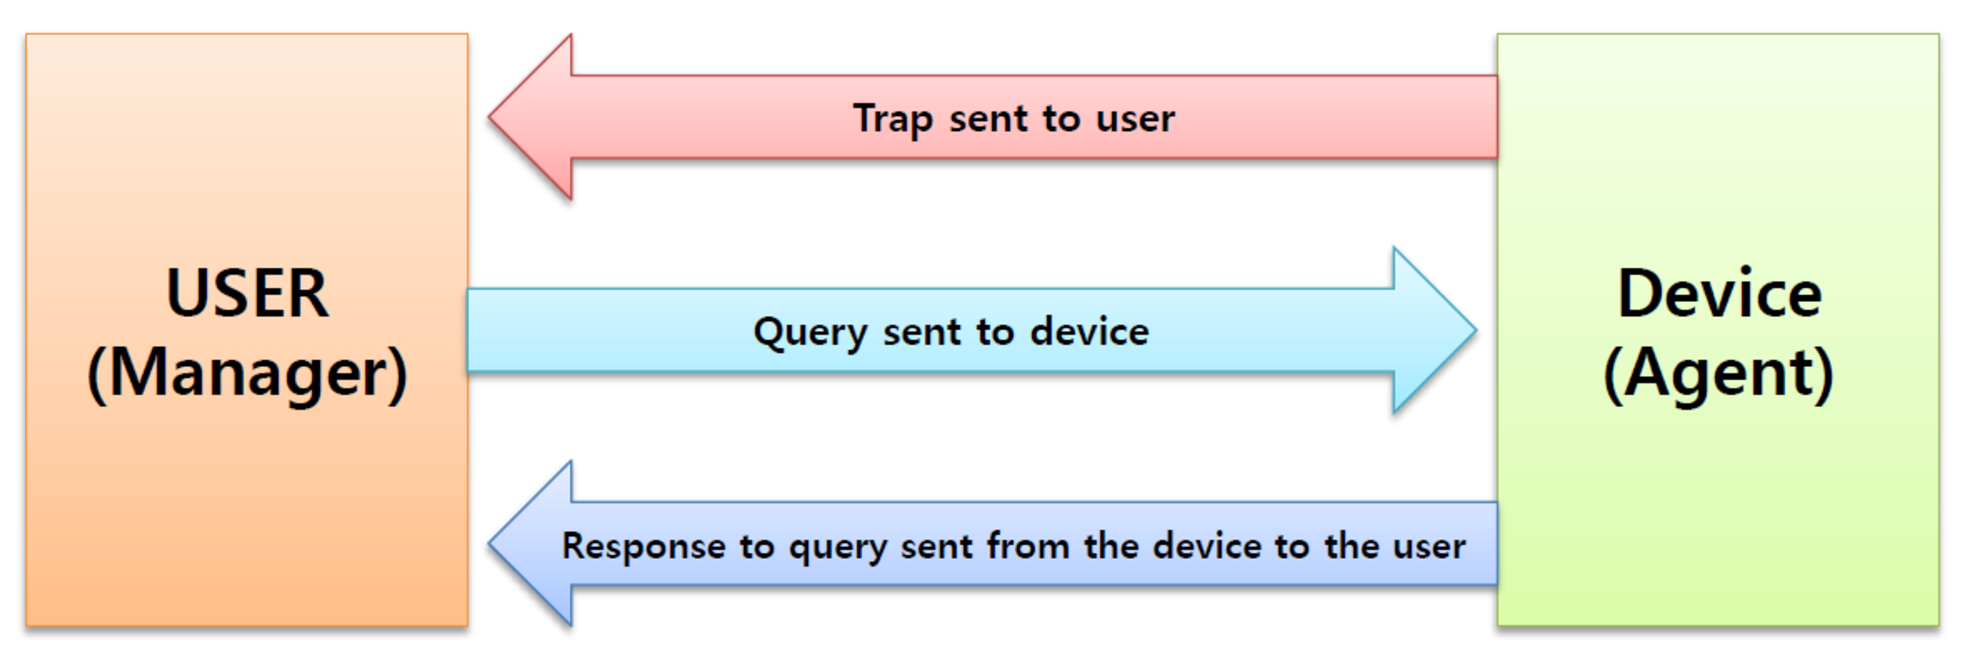
\includegraphics[width=0.65\textwidth]{./images/relationship_m_a.eps}
  \caption{Manager와 Agent의 관계}
  \label{fig:relationship_m_a}   
\end{figure}

\hfill

\section{EPICS}
EPICS (Experimental Physics and Industrial Control System)는 Los Alamos국립 연구소와, Argonne국립 연구소에서 공동개발 되어 오픈 라이센스로 제공되는 실시간 분산 제어 시스템으로 네트워크로 연결된 다양한 장비들의 모니터링 및 제어를 위해 사용된다. EPICS는 현재 전 세계 과학시설의 개발자들에 의해 개발이 진행되고 있다. EPICS는 그림 \ref{fig:ca}의 EPICS 로고와 같이 네트워크 기반의 클라이언트/서버 구조이며, TCP/UDP 프로토콜을 사용하는 CA (Channel Access) 통신 프로토콜을 사용하여 IOC (Input Output Controllers)를 통해 PV (Process Variable)를 주고 받는다. 클라이언트는 PV에 접근하며, 서버는 PV에 대한 접근을 제공한다. 특히, CA는 높은 대역폭, soft real-time networking 제어가 요구되는 응용프로그램들에 맞춰 설계되었고, 이는 엄청난 수의 컴퓨터와 장비들을 포함한 제어시스템 구축에 EPICS가 사용될 수 있는 이유이다. 또한 EPICS는 신뢰성 레벨을 제공하며, 이미 구축된 시스템의 유지보수가 용이하다는 장점이 있다\citep{epics}. 

\begin{figure}[h!]
  \centering
  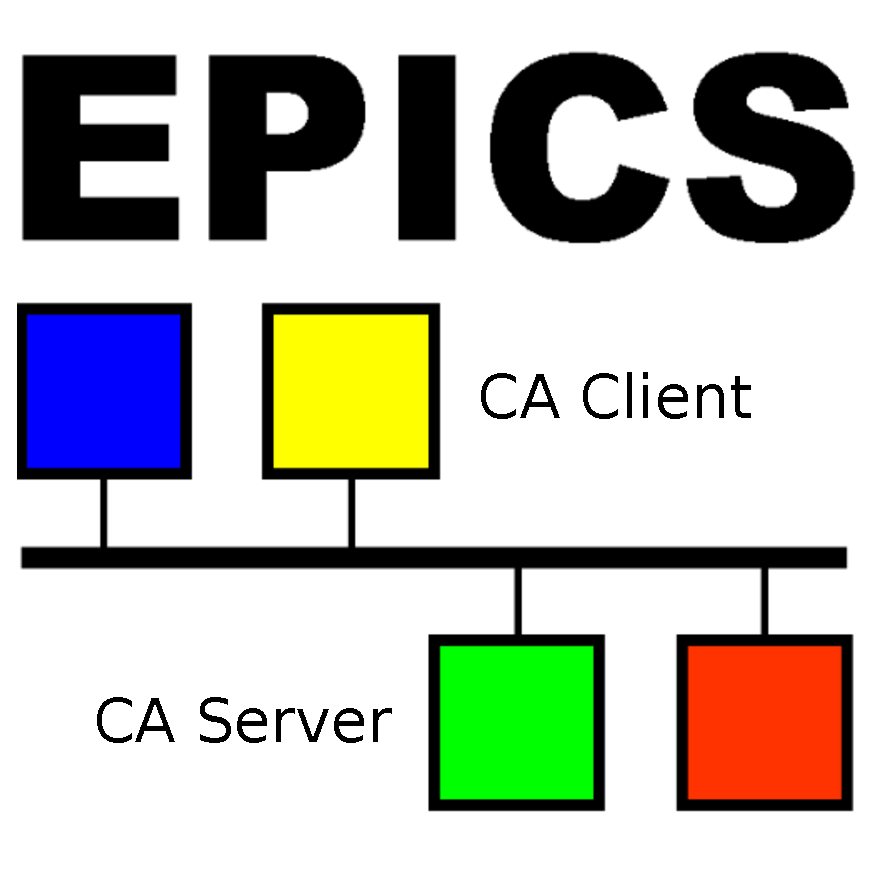
\includegraphics[width=0.3\textwidth]{./images/epics.eps}
  \caption{Channel Access 구조}
  \label{fig:ca}     
\end{figure}

\section{EPICS와 SNMP의 통합}
EPICS와 통합된 네트워크 기반의 제어 시스템 구축에 SNMP가 용이한 이유는 가속기 제어 시스템에 사용 될 장비와 장치들은 Ethernet환경을 통해 연결되며, 대부분 SNMP를 지원하기 때문이다. 따라서, EPICS와 SNMP의 통합은 중이온가속기 중앙 제어 시스템의 일관성, 유지관리의 용이성, 그리고 최적화 기술의 습득 및 축적의 관점에서 중요하다. 그림 \ref{fig:architecture}은 EPICS와 SNMP 통합 시스템의 구조로, 통합 시스템에서 모니터링 및 제어 될 장비는 SNMP MIB를 통해 EPICS와 연결되고, 이는 IOC로 개발되어 CA를 통한 PV와 장비의 통신을 가능하게 한다. PV는 MIB가 가진 장비의 정보로 모니터링 및 제어에 사용된다\citep{epicssnmp}. 

\begin{figure}[h!]
  \centering
  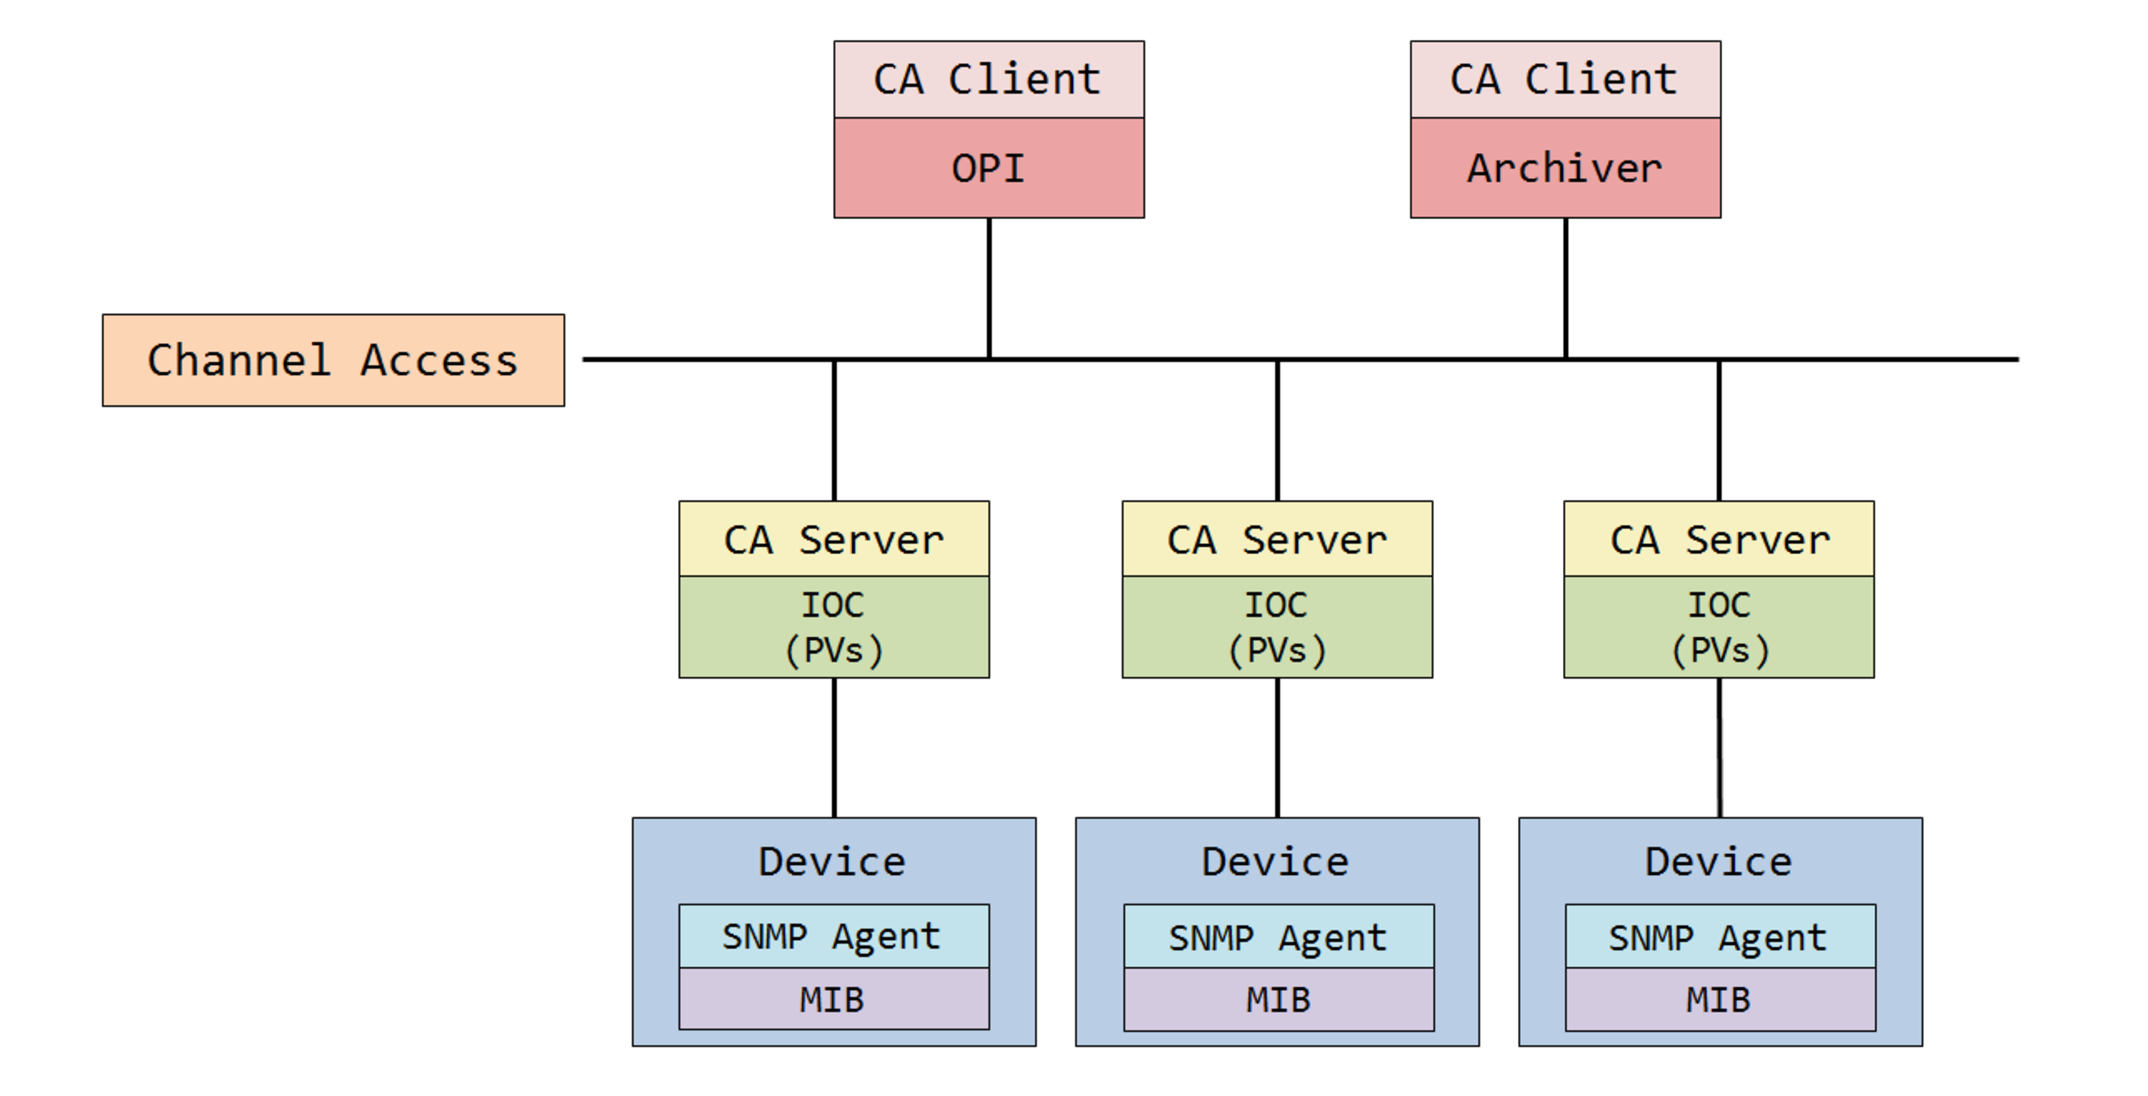
\includegraphics[width=0.89\textwidth]{./images/architecture.eps}
  \caption{EPICS와 SNMP 통합 시스템 아키텍쳐}
  \label{fig:architecture}   
\end{figure}

\chapter{EPICS IOC Support Modules}
EPICS IOC Support Module은 다른 종류의 인터페이스를 가진 하드웨어에 따라 새로운 타입의 레코드나 소프트웨어를 지원하는 Module인 Soft Support와 IOC내에서 사용 가능한 하드웨어를 지원하는 Module인 Hardware Support로 분류되어 제공된다. SNMP Soft Support Module은 이미 다수의 개발자들에 의해 devSNMP와 이를 보완한 snmp-nscl 등이 존재한다. 본 연구에서는 NSCL/FRIB의 SNMP Device Support Module(snmp-nscl)을 사용하여 초기 버전의 모니터링 시스템을 구축한다\citep{modules}.

\section{NSCL/FRIB SNMP Device Support Module}
NSCL/FRIB SNMP Device Support Module (이하 snmp-nscl)은 EPICS와 SNMP를 통한 하드웨어 장비와의 통신을 위해 2004년 LANL (Los Alamos National Laboratory)의 Richard Dubney에 의해 최초 개발 된 후 DESY (Deutsches Elektronen-Synchrotron)의 Albert Kagarmanov에 의해 개발된 devSNMP를 기반으로 NSCL (National Superconducting Cyclotron Laboratory)/FRIB (Facility for Rare Isotope Beams)의 John Priller에 의해 개발되었다. DESY의 devSNMP는 snmpv1/2c와 snmp Read만을 지원했다. 이에 devSNMP의 코드를 기반으로 snmpv1/2c/3과 snmpRead/ Write를 지원하는 snmp-nscl이 개발되었다. 이는 현재 Wiener/ISEG/MPOD power supply crates에 초점을 두고 RC9버전까지 개발되었으며, SNMPv2에 최적화 되어있다\citep{devsnmp}. 

\subsection{사용 방법}
snmp-nscl을 사용하여 SNMP를 통해 하드웨어와 EPICS가 통신하기 위해서는 Net-SNMP library와 SNMP를 지원하는 장비, 그리고 장비의 MIB파일이 필요하다. MIB는 보통 리눅스 시스템에서 아래의 경로에 있다.

\begin{lstlisting}[style=termstyle]
/usr/local/share/snmp/mibs/ 
/usr/share/mibs
\end{lstlisting}

하지만 일반적인 경로에 없을 경우, IOC st.cmd에 아래와 같이 epics환경변수로 MIB의 경로를 추가할 수 있다.

\begin{lstlisting}[style=termstyle]
epicsEnvSet("MIBDIRS", "+$(TOP)/mibs:/some/other/directory")
\end{lstlisting}

기본적인 설정을 끝낸 후, 장비를 모니터링 및 제어하기 위해서는 원하는 정보값 즉, MIB의 OID 객체를 Support Module의 Record로 정의하여야한다. 정의된 Record들은 db파일이 되어 장비와의 통신에 사용된다. Support Module은 snmp Read/Write에 따라 Input(ai, longin, stringin, waveform(DBF\_STRING, DBF\_CHAR, DBF\_UCHAR))과 Output(ao, longout, stringout)의 Record타입을 지원하며, Record의 포맷은 다음과 같다. 

\begin{lstlisting}[style=termstyle]
- SNMP Read
   record(ai, "$(DEV):VoltageRead")
   {
     field(DESC, "SNMP channel")
     field(DTYP, "Snmp")
     field(SCAN, ".2 second")
     field(PREC, "3")
     field(INP, "@$(HOST) guru WIENER-CRATE-MIB::outputMeasurementSenseVoltage.$(CHAN) Float: 100")
   }

- SNMP Write
   record(ao, "$(DEV):VoltageSet")
   {
     field(DESC, "SNMP channel")
     field(DTYP, "Snmp")
     field(SCAN, "Passive")
     field(PREC, "3")
     field(OUT, "@$(HOST) guru WIENER-CRATE-MIB::outputVoltage.$(CHAN) Float: 100 F")
   }
\end{lstlisting}

Record는 객체의 Read/Write여부에 맞춰 지정하고, 부가적인 설명과 테이터타입, 스캔시간에 대한 필드 값을 정의한다. 

\begin{lstlisting}[style=termstyle]
snmpget -v 2c -c public localhost RFC1213-MIB::sysName.0
\end{lstlisting}

이 때, INP/OUT 필드는 위의 snmpget 명령어와 유사한 포맷으로 원하는 장비의 hostname, community string, 객체의 이름 등을 아래와 같은 포맷으로 정의해야한다. 
\begin{lstlisting}[style=termstyle]
@host community OIDname mask dataLength [set_type[special_flags]]
\end{lstlisting}
여기서 mask는 정보 값의 데이터타입에 따라 정의되며, 제어 시에는 snmpset 명령어와 마찬가지로 set\_type을 데이터타입에 따라 정의하여야한다.\footnote{* 각 정보에 대한 설명은 devSNMP Documentation을 참조 바란다.} 이렇게 정의 된 db파일의 Record들은 PV가 되어 하드웨어와 EPICS의 통신에 사용된다.

\subsection{장단점}




\clearpage

\section{Device Support Module을 이용한 통합 시스템 구축}
본 문서에서는 SNMPv1/2c를 지원하는 snmp-nscl RC8버전을 사용하여 중이온가속기 제어 시스템 개발 환경에 맞춘 통합 모니터링 시스템 초기버전을 구축하였다. 구축된 모니터링 시스템은 가속기 제어 시스템에 사용되는 다양한 장비 적용에 앞서 사무실 내의 프린터기에 적용되었다. 프린터 모니터링 시스템 구축에 사용된 소프트웨어와 하드웨어는 다음과 같다.

\begin{itemize}
\item Debian Linux 7 Wheezy
\item NET-SNMP v5.4.3
\item EPICS v3.14.12.4
\item FRIB SNMP Device Support Module RC8
\item EPICS CSS (Control System Studio)
\item Printers (XEROX ApeosPort-IV C3375, KYOCERA FS-9530DN)
\end{itemize}

\subsection{Customize 이유 및 수정 사항}
중이온가속기 제어 환경은 각 시스템의 원활한 개발을 위하여 EPICS 개발 환경이 표준화 되어있으며\citep{epicsev}, 표준화된 EPICS 기본 구조는 그림 \ref{fig:epicstree}와 같다.

\begin{figure}[h!]
  \centering
  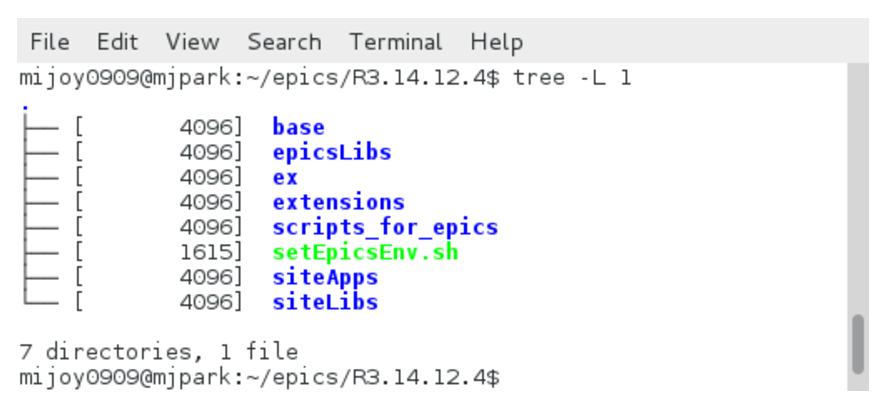
\includegraphics[width=0.6\textwidth]{./images/epicstree.eps}
  \caption{중이온가속기 제어 환경의 EPICS 기본 구조}
  \label{fig:epicstree}   
\end{figure}


\clearpage
표준화 된 중이온가속기 제어 개발 환경과 프린터 모니터링에 최적화하기 위해 그림 \ref{fig:fribtree}의 구조를 가진 snmp-nscl의 아래와 같은 사항들이 수정되었다.

\begin{figure}[h!]
  \centering
  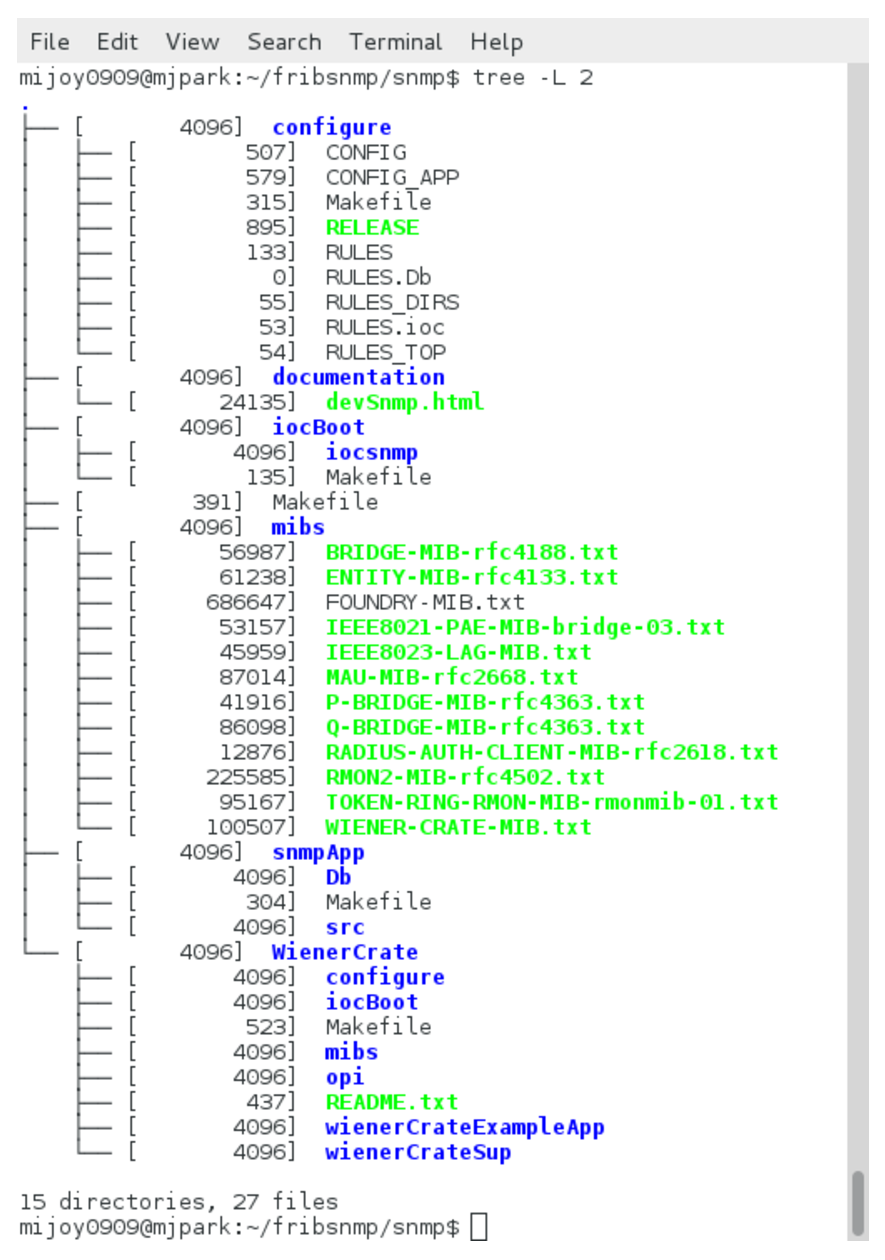
\includegraphics[width=0.6\textwidth]{./images/fribmoduletree.eps}
  \caption{FRIB SNMP Device Support Module의 구조}
  \label{fig:fribtree}  
\end{figure}

\begin{enumerate}
\item 표준화된 중이온가속기 제어 환경에 맞춰 Library (siteLibs)와 Application (siteApps)으로 분리\\
- 기존의 snmp-nscl은 통합된 Library와 Application을 가지고 있었으나, 그림 \ref{fig:makesitelib_frib}, \ref{fig:makesiteapp_frib}과 같이 Module의 Makefile 수정 및 파일 이동의 과정을 거쳐 가속기 제어 개발 환경에 맞게 siteLibs(그림 \ref{fig:sitelib_frib})과 siteApps(그림 \ref{fig:siteapp_frib})로 분리시켰다.

\begin{figure}[!h]
  \centering
  \subbottom[Labrary Makefile]
  	    {
  	      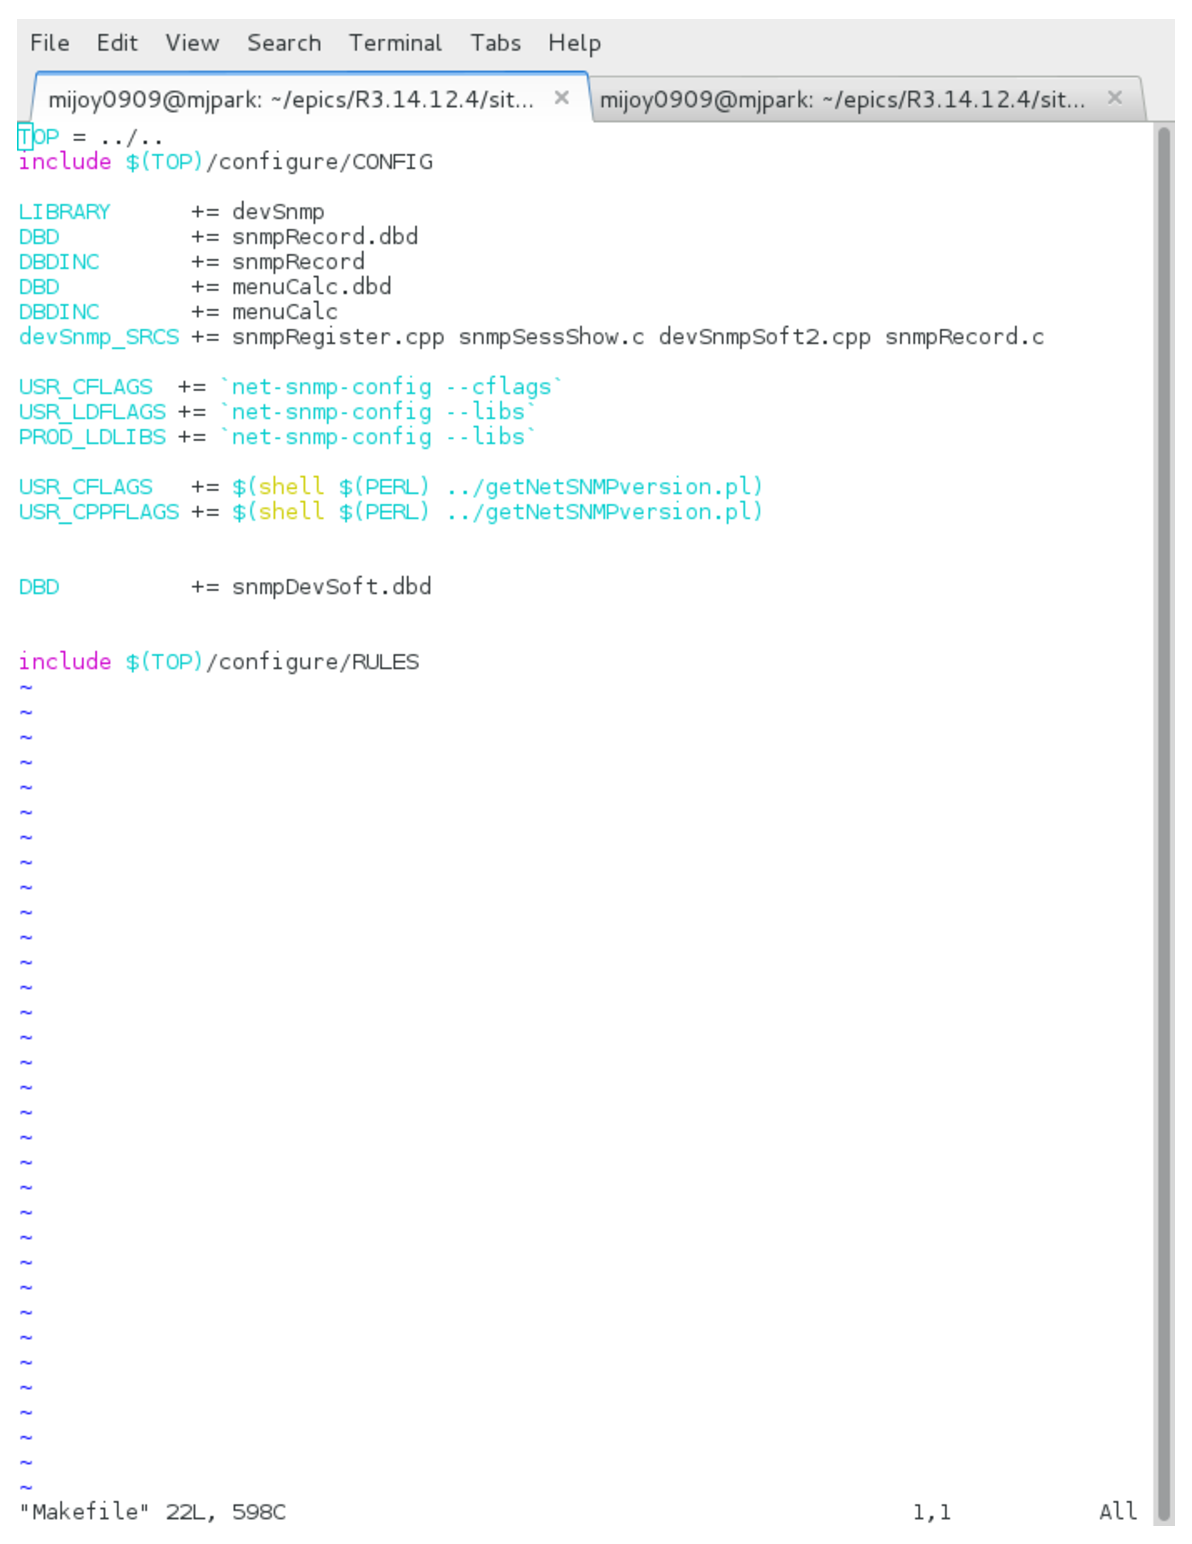
\includegraphics[width=0.45\textwidth]{./images/fribmake_lib.eps}
  	      \label{fig:makesitelib_frib}
  	    }
              \hfill
  \subbottom[Application Makefile]
  	    {
  	      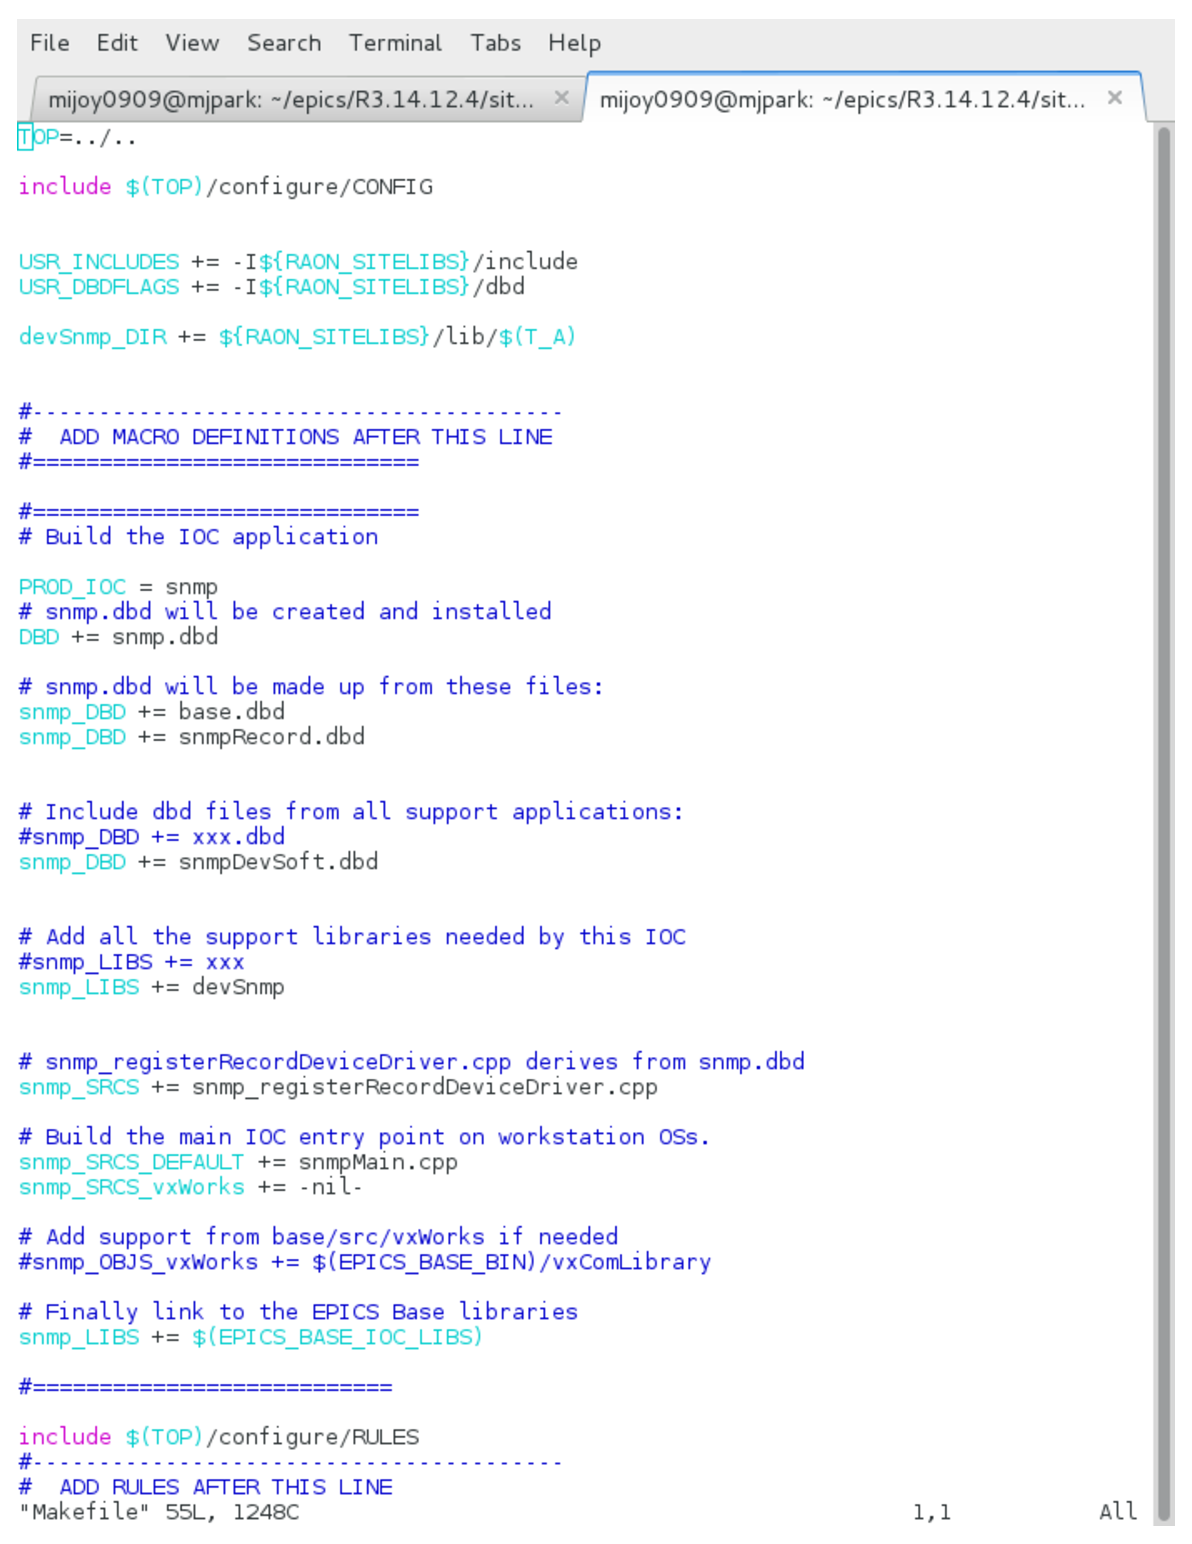
\includegraphics[width=0.45\textwidth]{./images/fribmake_app.eps}
  	      \label{fig:makesiteapp_frib}
  	    }
              \hfill
            
\subbottom[SiteLibs]
	    {
	      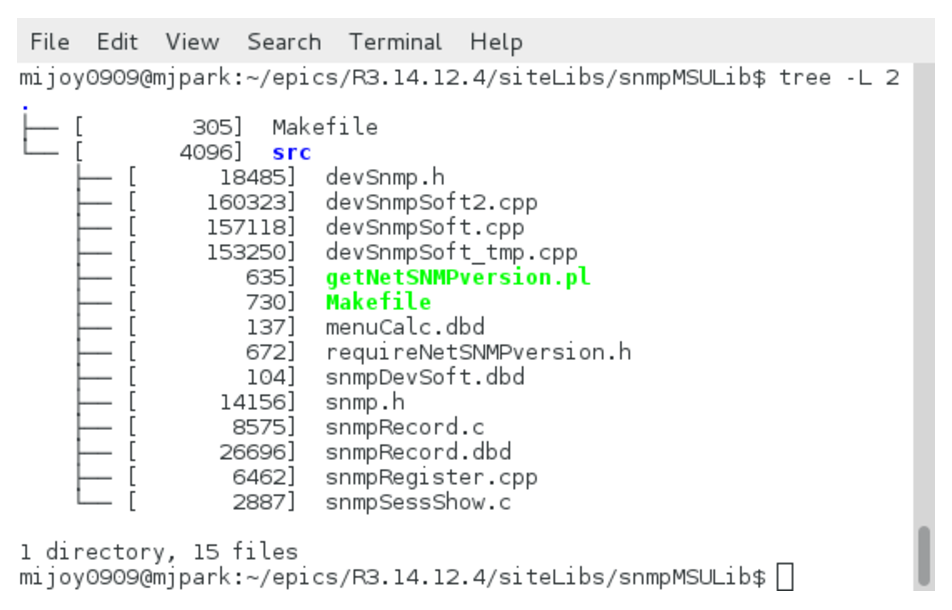
\includegraphics[width=0.45\textwidth]{./images/sitelib_frib.eps}
	      \label{fig:sitelib_frib}
	    }
            \hfill
\subbottom[SiteApps]
	    {
	      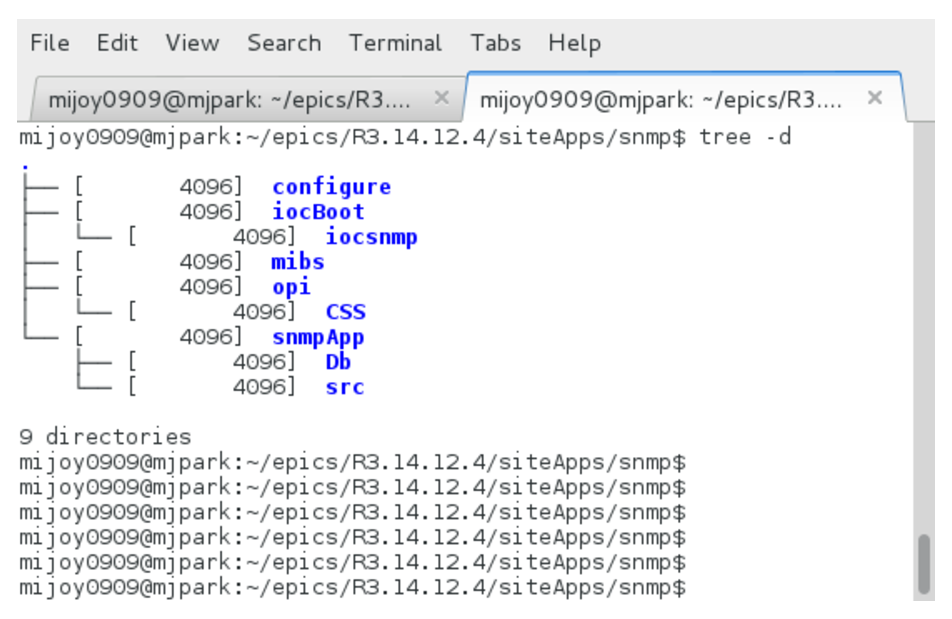
\includegraphics[width=0.45\textwidth]{./images/siteapp_frib.eps}
	      \label{fig:siteapp_frib}
	    }
            \hfill
\subbottom[snmpRecord]
	    {
	      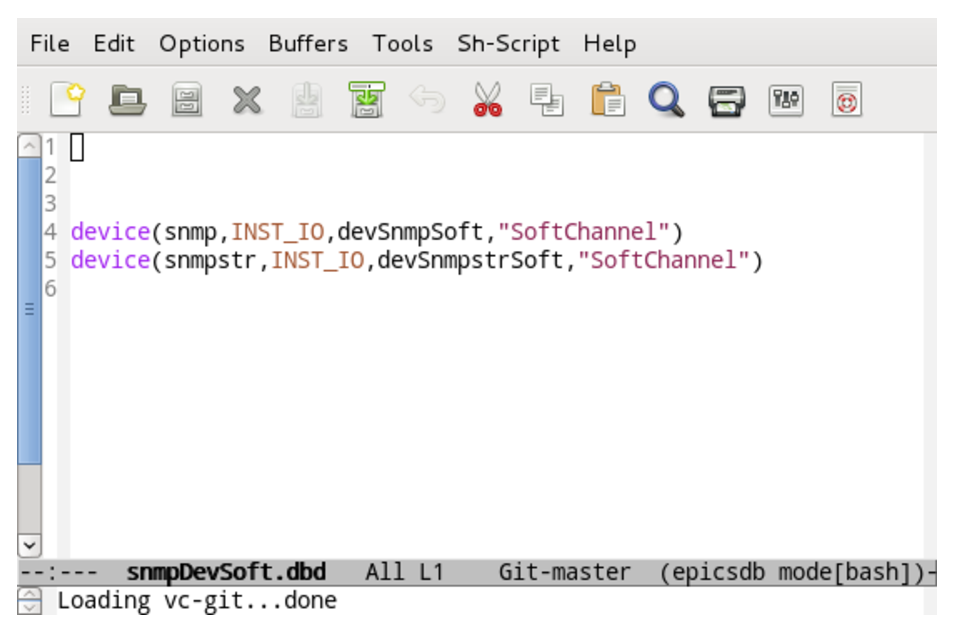
\includegraphics[width=0.45\textwidth]{./images/frib_snmprecord_dbd.eps}
	      \label{fig:frib_snmprecord_dbd}
 	    }
 	                \hfill
\subbottom[calc source code]
	    {
	      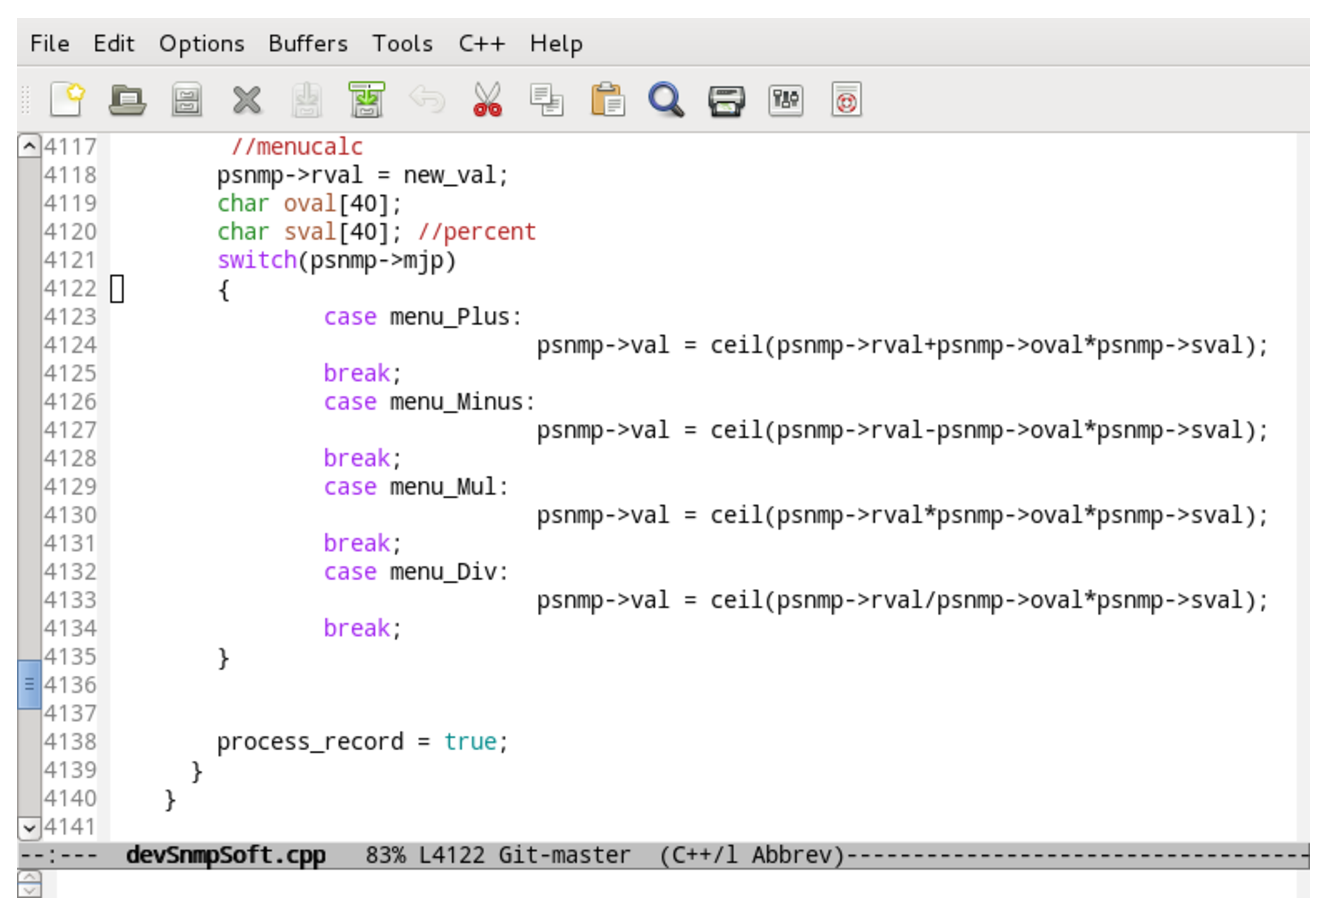
\includegraphics[width=0.45\textwidth]{./images/frib_calccode.eps}
	      \label{fig:frib_calccode}
	    }
	                \hfill
  \caption
      {
        중이온가속기 제어 개발 환경에 맞춰 수정된 SNMP Device Support Module 
      }
 \label{fig:frib_raon}
\end{figure}

\clearpage
\item 기존의 여러 종류의 Support Module에서 제공하는 Record를 대신하여 통합 시스템에서 사용 될 snmpRecord, snmpstrRecord 생성(그림 \ref{fig:frib_snmprecord_dbd})
\item 가독성 측면에서 프린터의 종이, 잉크의 잔량은 퍼센트로 나타내기 위해 siteLibs내 소스코드에 사칙연산 코드 추가 및 Record내 MJP필드 생성(그림 \ref{fig:frib_calccode})
\end{enumerate}

\begin{figure}[h!]
  \centering
  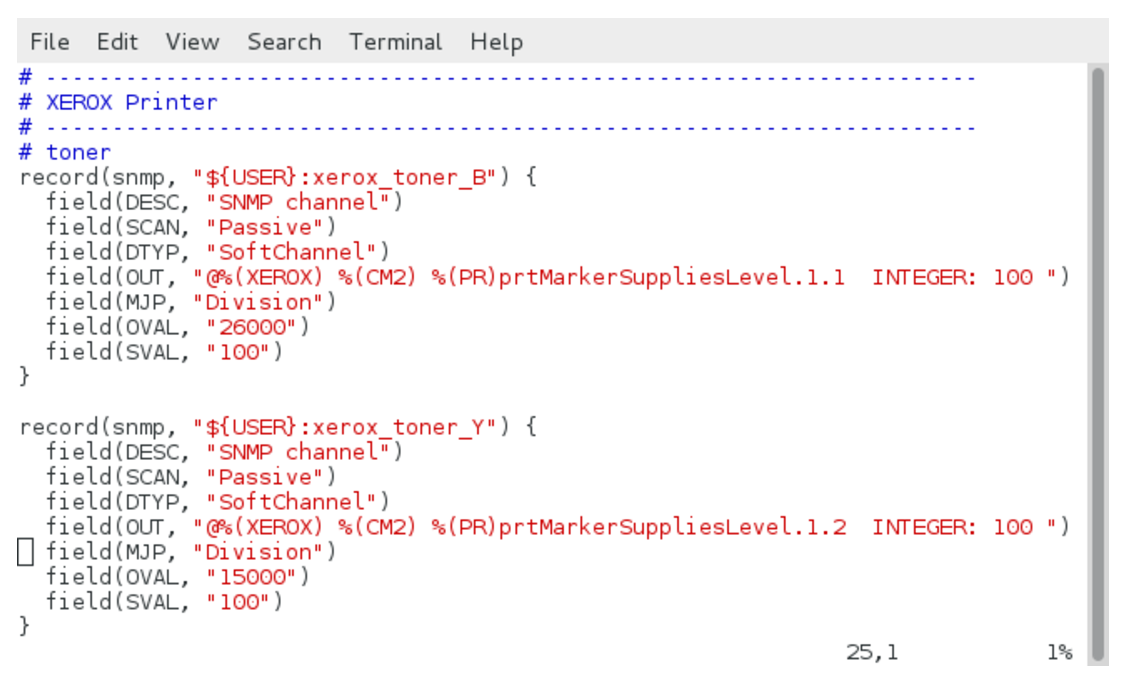
\includegraphics[width=0.7\textwidth]{./images/app.eps}
  \caption{EPICS DB파일}
  \label{fig:db}   
\end{figure}

이렇게 그림 \ref{fig:frib_raon}과 같이 수정된 Module을 사용하여 통합 장비 모니터링 시스템 구축을 위해서는 siteApps내에 그림 \ref{fig:db}과 같이 DB파일을 생성하고 IOC를 실행시키면 각 Record는 EPICS IOC내 PV가 되어 아래와 같이 CA 통한 프린터기 모니터링이 가능해진다. 

\begin{figure}[h!]
  \centering
  	      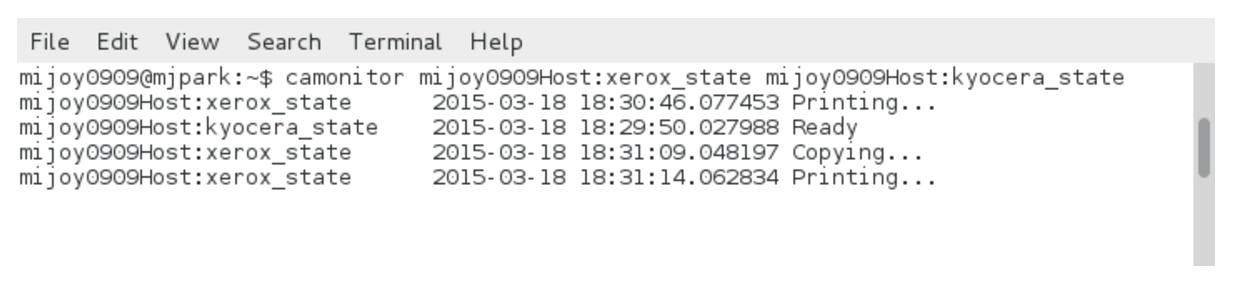
\includegraphics[width=0.89\textwidth]{./images/printer_camoni.eps}
  \caption{camonitor}
  	      \label{fig:printer_camoni}
\end{figure}

\clearpage

\begin{figure}[h!]
  \centering
  	      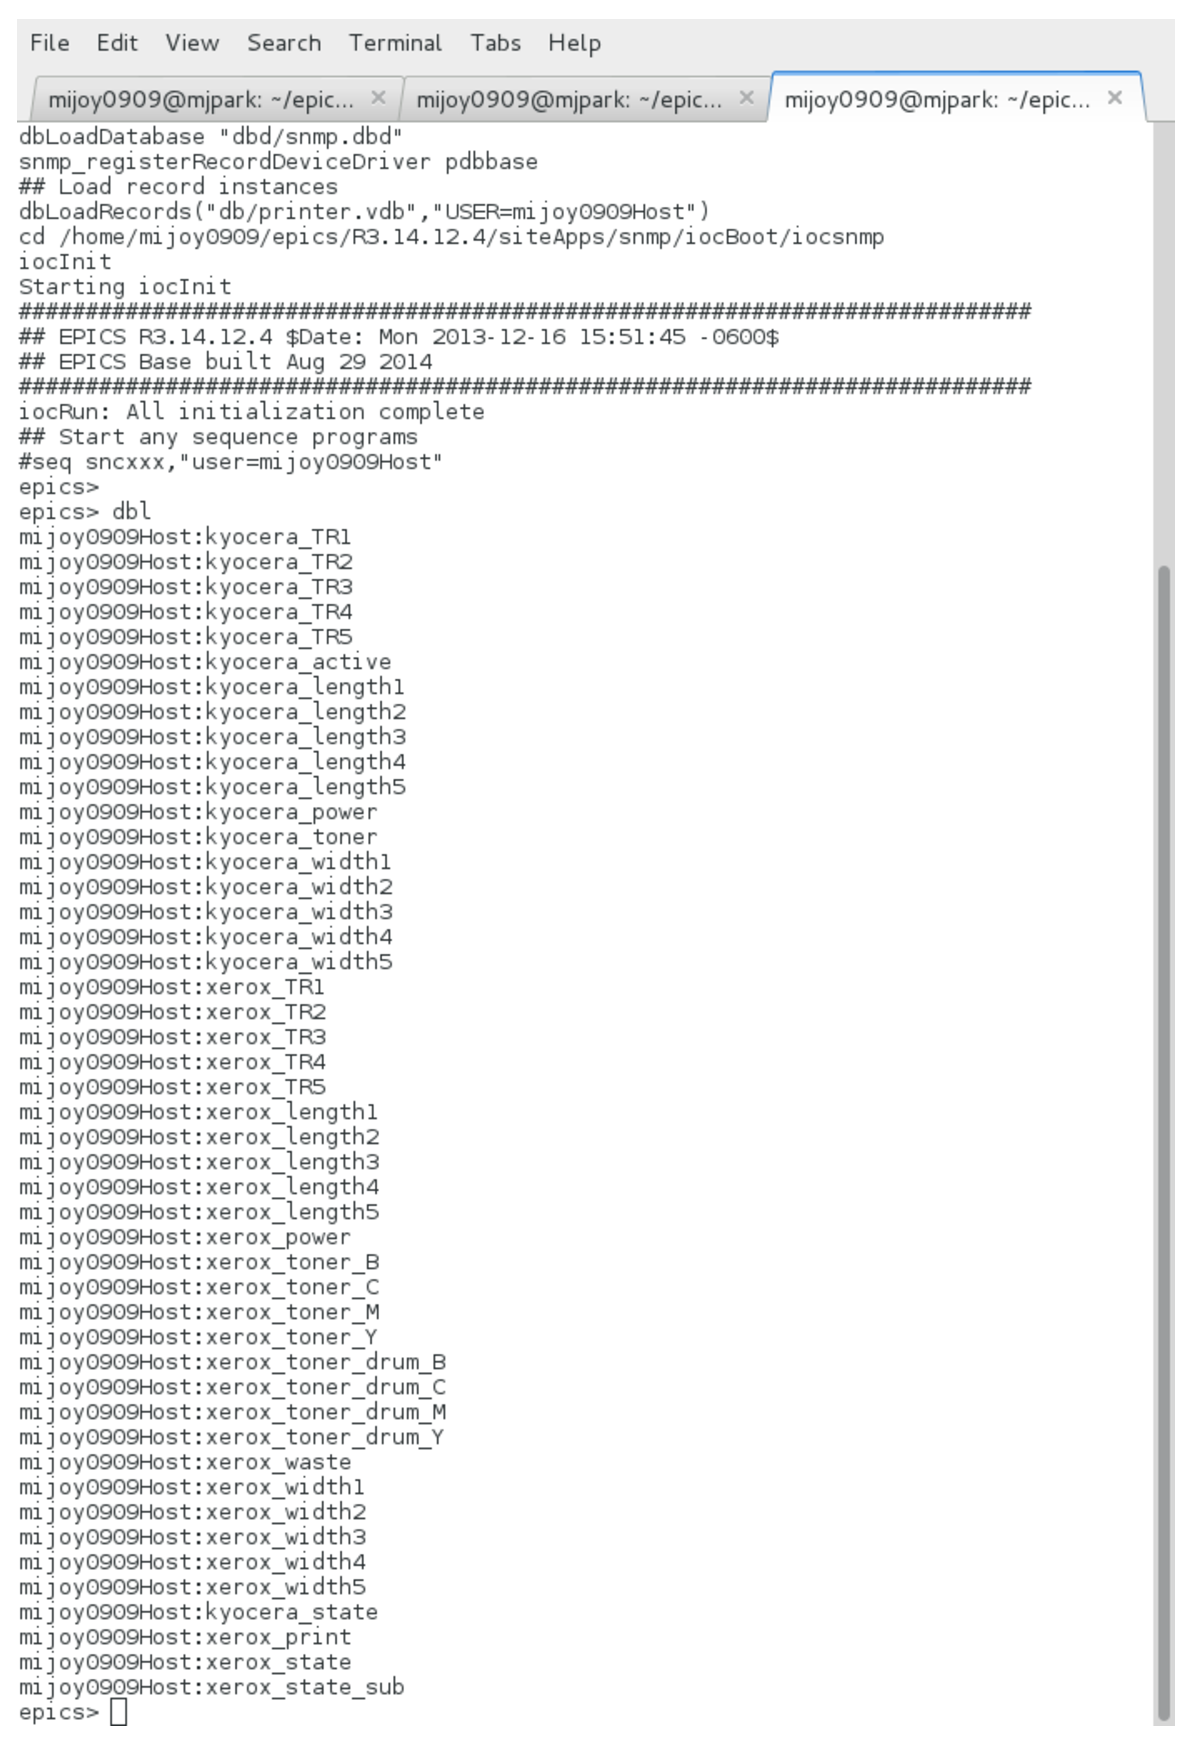
\includegraphics[width=0.89\textwidth]{./images/printer_ioc.eps}
  \caption{EPICS IOC 실행 및 PV 리스트}
  	      \label{fig: printer_ioc}
\end{figure}

각각의 PV들은 EPICS의 UI (User Interface)프로그램인 CSS (Control System Studio)를 사용하여 프린터 모니터링 시스템의 OPI (Operator Interface)로 구현되고, 이 OPI는 현재 그림 \ref{fig:css_monitoring}과 같이 프린터의 상태, 종이량 등의 정보 및 사무실 환경 모니터링에 사용되고 있다.

\begin{figure}[h!]
  \centering
  \includegraphics[width=0.89\textwidth]{./images/css_monitoring.eps}
  \caption{EPICS DB파일}
  \label{fig:css_monitoring}   
\end{figure}

\clearpage

\chapter{Legacy SNMP Code}
\section{Net-snmp tutorial}




\clearpage
\bibliographystyle{unsrtnat}
\bibliography{./refs}




\end{document}
